\chapter{RMN em profundidade: pulsos, relaxação e 2D}\label{ch:b3:advanced-nmr}

Um aparelho de ressonância magnética de hospital e o espectrômetro de RMN de
um departamento de química funcionam segundo o mesmo princípio. Cada um põe
núcleos de hidrogênio em um campo magnético intenso, inclina sua magnetização
com um pulso curto de ondas de rádio e escuta o fraco sinal que ela induz
enquanto precessiona e relaxa. O aparelho transforma o sinal em uma imagem
dos tecidos moles; o espectrômetro, em uma lista de deslocamentos químicos e
acoplamentos e, com vários pulsos seguidos, em mapas bidimensionais que
mostram qual átomo está ligado a qual. Este capítulo explica o que fazem os
pulsos, por que o sinal se apaga e como se leem os \omterm{def:b3:advanced-nmr:two-d}{espectros bidimensionais}
--- o método pelo qual hoje se resolve a maioria das novas estruturas orgânicas.

\begin{recall}
O volume do 1.º ano interpretou espectros de RMN de ${}^1$H: deslocamento
químico, blindagem, prótons equivalentes, integração, acoplamento spin--spin,
constantes de acoplamento e multipletos. O volume do 2.º ano acrescentou a
RMN de ${}^{13}$C com desacoplamento de banda larga e o DEPT, cuja sequência de
pulsos tomou como dada; os pulsos são explicados aqui. O
\cref{ch:b3:many-electron-atoms} tratou o spin como um momento angular. Da
física: um momento magnético em um campo tem energia $-\boldsymbol\mu\cdot\mathbf B$, e
as populações dos níveis seguem o fator de Boltzmann $\eu^{-\Delta E/kT}$,
desenvolvido no \cref{ch:b3:partition-functions}.
\end{recall}

\begin{omfigure}
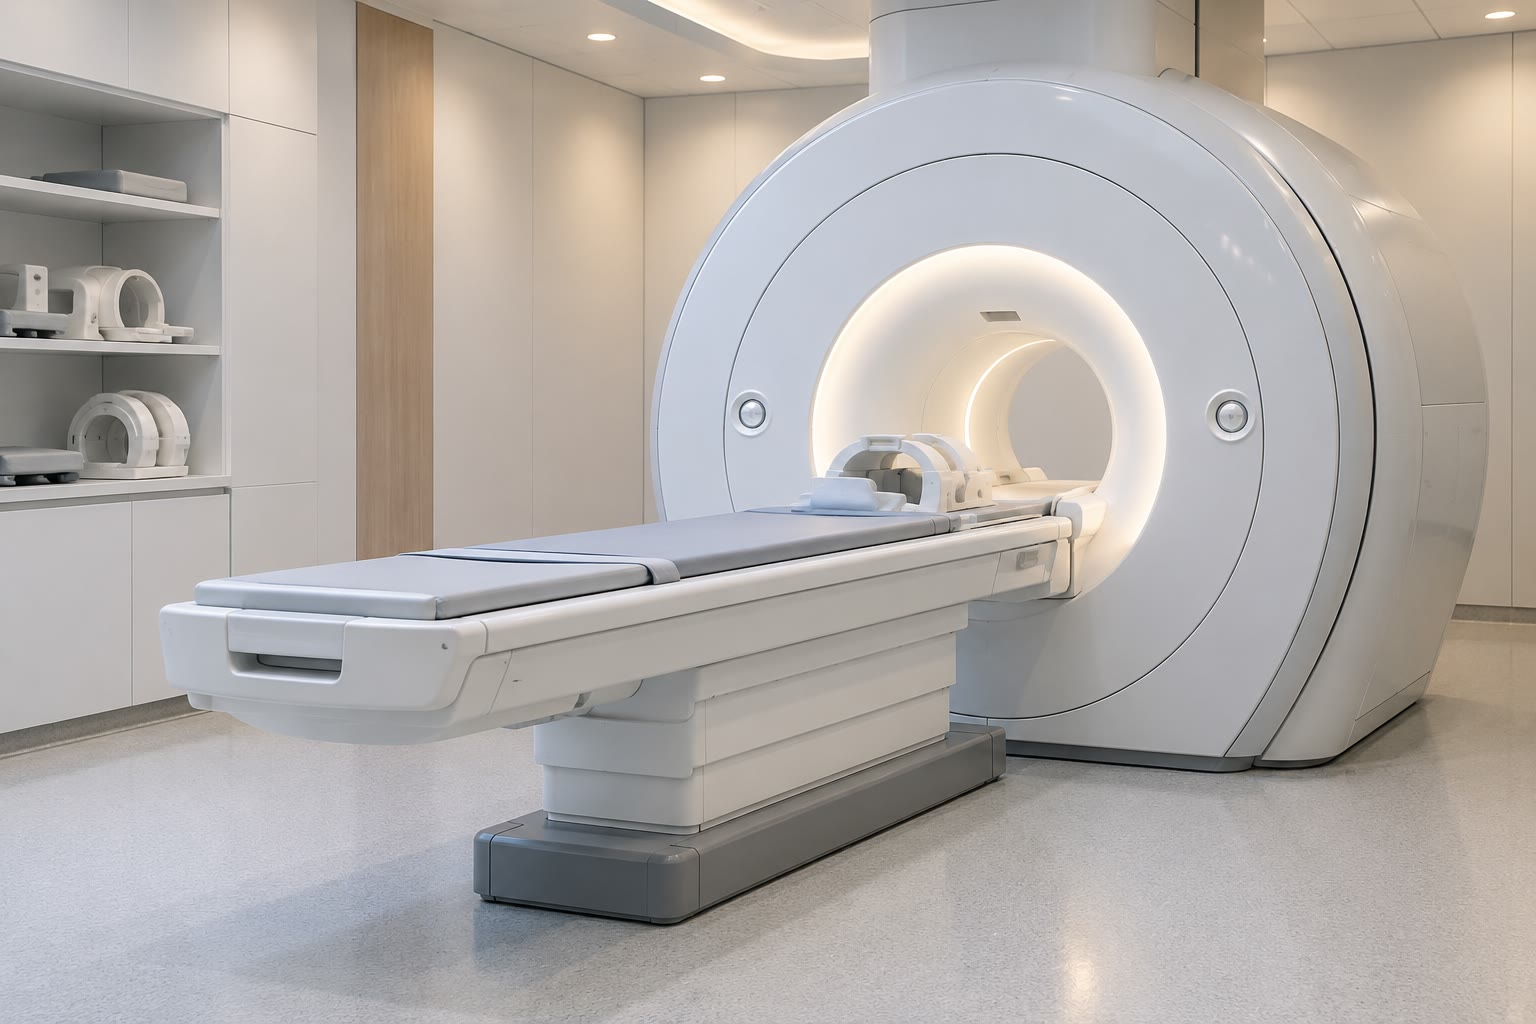
\includegraphics[width=0.52\linewidth]{images/book4/ai/b3-08-mri.jpg}\hspace{0.8em}%
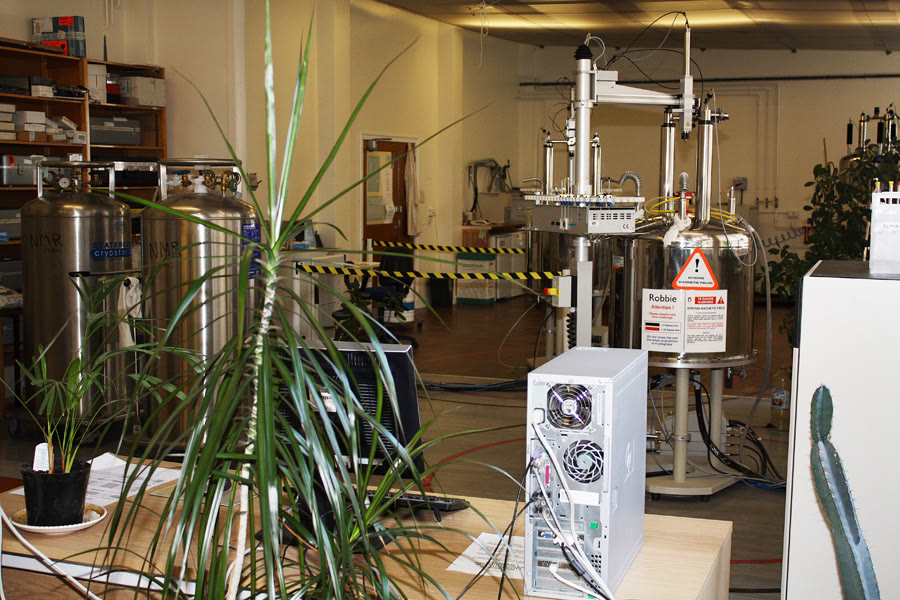
\includegraphics[width=0.4\linewidth]{images/book4/nmr-lab.jpg}

{\small À esquerda: um aparelho de ressonância magnética de hospital. À
direita: um laboratório de RMN; cada ímã supercondutor fica em seu criostato,
reabastecido com hélio líquido e nitrogênio líquido a partir dos dewars à
esquerda. Fotografia de Shandchem, CC BY 2.0.}
\end{omfigure}

\section{Spins nucleares em um campo magnético}

\begin{definition}[Número quântico de spin nuclear, razão giromagnética]\label{def:b3:advanced-nmr:nuclear-spin}
Um núcleo tem um momento angular de spin de número quântico $I$, seu
\emph{número quântico de spin nuclear}\index{numero quantico de spin nuclear@número quântico de spin nuclear} ($I = 0$
para \ce{^{12}C}, \ce{^{16}O}; $\frac12$ para \ce{^1H}, \ce{^{13}C}, \ce{^{15}N}, \ce{^{19}F},
\ce{^{31}P}; 1 para \ce{^2H}, \ce{^{14}N}), e um momento magnético $\boldsymbol\mu = \gamma\hat{\mathbf
I}$ proporcional a ele; $\gamma$ é a \emph{razão giromagnética}\index{razao giromagnetica@razão giromagnética}.
Ao longo de um campo $B_0$ (eixo $z$), $\hat I_z$ assume os valores $m_I\hbar$,
$m_I = -I, \dots, I$.
\end{definition}

\begin{proposition}[Níveis Zeeman]\label{prop:b3:advanced-nmr:zeeman}
Em um campo $B_0$, os níveis são $E_m = -m_I\gamma\hbar B_0$; as transições $\Delta m_I = \pm1$
absorvem na frequência
\[
\nu_0 = \frac{\gamma B_0}{2\pi}.
\]
\end{proposition}

\begin{proof}
$E = -\boldsymbol\mu\cdot\mathbf B = -\gamma B_0\hat I_z$, de \omterm{def:b3:quantum-model-systems:operator}{autovalores} $-\gamma B_0m_I\hbar$. Níveis
adjacentes diferem de $\gamma\hbar B_0 = h\nu_0$.
\end{proof}

\begin{definition}[Frequência de Larmor]\label{def:b3:advanced-nmr:larmor}
$\nu_0 = \gamma B_0/2\pi$ é a \emph{frequência de Larmor}\index{frequencia de Larmor@frequência de Larmor} do
núcleo: a frequência da ressonância e também a frequência com que seu
momento magnético precessiona em torno do campo.
\end{definition}

\begin{example}[Os núcleos comuns]\label{ex:b3:advanced-nmr:nuclei}
% ledger: const:gammaP, nuc:C13.mu, nuc:F19.mu, nuc:P31.mu, nuc:N15.mu, const:muN
Para um núcleo de spin $\frac12$ e momento $\mu$, $\gamma/2\pi = \mu/(Ih) = 2\mu/h$. Com os
momentos medidos: \ce{^1H} \qty{42.58}{MHz/T}, \ce{^{19}F} \qty{40.08}{MHz/T}, \ce{^{31}P}
\qty{17.25}{MHz/T}, \ce{^{13}C} \qty{10.71}{MHz/T}, \ce{^{15}N} \qty{-4.32}{MHz/T}. Um
``espectrômetro de \qty{400}{MHz}'' tem $B_0 = \qty{9.4}{T}$: seus prótons ressoam em
\qty{400.2}{MHz}, seus carbonos em \qty{100.7}{MHz}.
\end{example}

\begin{proposition}[Uma diferença de população ínfima]\label{prop:b3:advanced-nmr:populations}
Para spin $\frac12$ à temperatura $T$, o excesso de núcleos no nível inferior é
\[
\frac{N_\alpha - N_\beta}{N} \approx \frac{\gamma\hbar B_0}{2kT}.
\]
\end{proposition}

\begin{proof}
$N_\beta/N_\alpha = \eu^{-\Delta E/kT} \approx 1 - \Delta E/kT$, pois $\Delta E \ll kT$; logo
$(N_\alpha - N_\beta)/(N_\alpha + N_\beta) \approx \Delta E/2kT$, com $\Delta E = \gamma\hbar B_0$.
\end{proof}

Para prótons a \qty{9.4}{T} e \qty{300}{K}, o excesso é \num{3.2e-5}: apenas
três núcleos em cem mil contribuem. Como o excesso e a tensão induzida na
bobina crescem ambos com $\gamma$ e $B_0$, o sinal cresce aproximadamente
como $\gamma^3B_0^2$: é a razão de ímãs cada vez mais intensos e da baixa
sensibilidade dos núcleos de $\gamma$ pequeno e baixa abundância natural, como o
\ce{^{13}C}.

\section{Pulsos e o decaimento de indução livre}

\begin{definition}[Magnetização resultante, referencial girante]\label{def:b3:advanced-nmr:magnetisation}
A \emph{magnetização resultante}\index{magnetizacao resultante@magnetização resultante} $\mathbf M$ de uma amostra é a
soma de seus momentos magnéticos nucleares por unidade de volume; no equilíbrio, ela é
$M_0$ ao longo de $\mathbf B_0$. O \emph{referencial girante}\index{referencial girante} é um sistema
de eixos $x'$, $y'$, $z$ que gira em torno de $z$ com a frequência das ondas de
rádio aplicadas; nele, a precessão em $\nu_0$ aparece desacelerada até o desvio $\nu_0 -
\nu_{\mathrm{rf}}$.
\end{definition}

\begin{proposition}[Precessão]\label{prop:b3:advanced-nmr:precession}
Uma magnetização em um campo obedece a $\dd\mathbf M/\dd t = \gamma\,\mathbf M\times\mathbf B$; em um
campo estático $B_0\mathbf e_z$, sua componente transversal gira em torno de $z$ com a frequência
angular $\omega_0 = \gamma B_0$, enquanto $M_z$ permanece constante.
\end{proposition}

\begin{proof}[Demonstração parcial]
A equação é a equação clássica do torque para um momento magnético que
carrega momento angular, admitida da física. Com $\mathbf B = B_0\mathbf e_z$: $\dot M_x = \gamma
B_0M_y$, $\dot M_y = -\gamma B_0M_x$, $\dot M_z = 0$, cuja solução é $M_x + \iu M_y \propto
\eu^{-\iu\gamma B_0t}$: uma rotação em $\omega_0$ (no sentido horário visto de $+z$ para $\gamma > 0$).
\end{proof}

\begin{definition}[Pulso de radiofrequência, ângulo de nutação]\label{def:b3:advanced-nmr:pulse}
Um \emph{pulso de radiofrequência}\index{pulso de radiofrequencia@pulso de radiofrequência} é uma breve emissão de
ondas de rádio em $\nu_{\mathrm{rf}} \approx \nu_0$, cujo campo magnético $B_1$, fixo no
\omterm{def:b3:advanced-nmr:magnetisation}{referencial girante} ao longo de $x'$, gira $\mathbf M$ em torno de $x'$. O ângulo girado é o
\emph{ângulo de nutação}\index{angulo de nutacao@ângulo de nutação} $\theta = \gamma B_1t_p$ para um pulso de duração
$t_p$: um pulso de $90^\circ$ leva $\mathbf M$ ao plano $x'y'$, um pulso de $180^\circ$ o
inverte.
\end{definition}

\begin{omfigure}
\tdplotsetmaincoords{70}{120}
\begin{tikzpicture}[tdplot_main_coords, font=\small, >=Stealth]
  \begin{scope}
    \draw[->, gray] (0,0,0) -- (1.8,0,0) node[anchor=north east] {$x'$};
    \draw[->, gray] (0,0,0) -- (0,1.8,0) node[anchor=north west] {$y'$};
    \draw[->, gray] (0,0,0) -- (0,0,1.8) node[anchor=south] {$z$, $\mathbf B_0$};
    \draw[->, omThm, very thick] (0,0,0) -- (0,0,1.4) node[anchor=west] {$\mathbf M$};
    \node[anchor=north] at (0,0,-0.9) {equilíbrio};
  \end{scope}
  \begin{scope}[shift={(0,4.6,0)}]
    \draw[->, gray] (0,0,0) -- (1.8,0,0) node[anchor=north east] {$x'$};
    \draw[->, gray] (0,0,0) -- (0,1.8,0) node[anchor=north west] {$y'$};
    \draw[->, gray] (0,0,0) -- (0,0,1.8) node[anchor=south] {$z$};
    \draw[->, omDef, thick] (0,0,0) -- (1.2,0,0) node[anchor=south east, xshift=-2pt] {$\mathbf B_1$};
    \draw[->, omThm, very thick] (0,0,0) -- (0,1.4,0) node[anchor=south west] {$\mathbf M$};
    \node[anchor=north] at (0,0,-0.9) {após um pulso $90^\circ_{x'}$};
  \end{scope}
  \begin{scope}[shift={(0,9.2,0)}]
    \draw[->, gray] (0,0,0) -- (1.8,0,0) node[anchor=north east] {$x'$};
    \draw[->, gray] (0,0,0) -- (0,1.8,0) node[anchor=north west] {$y'$};
    \draw[->, gray] (0,0,0) -- (0,0,1.8) node[anchor=south] {$z$};
    \draw[->, omThm, very thick] (0,0,0) -- (0,0,-1.4) node[anchor=west] {$\mathbf M$};
    \node[anchor=north] at (0,0,-1.6) {após um pulso $180^\circ_{x'}$};
  \end{scope}
\end{tikzpicture}

{\small A magnetização no \omterm{def:b3:advanced-nmr:magnetisation}{referencial girante}. Um pulso de $90^\circ$ em torno de $x'$
gira $\mathbf M$ de $z$ para $y'$ (com $\gamma > 0$, a rotação segue a regra da
mão esquerda em torno de $\mathbf B_1$, a convenção usual); um pulso de $180^\circ$
a inverte.}
\end{omfigure}

\begin{definition}[Decaimento de indução livre]\label{def:b3:advanced-nmr:fid}
Depois de um pulso de $90^\circ$, a magnetização transversal precessiona na \omterm{def:b3:advanced-nmr:larmor}{frequência
de Larmor} e induz uma tensão oscilante na bobina em torno da amostra, que se
extingue à medida que a magnetização relaxa: é o \emph{decaimento de indução
livre}\index{decaimento de inducao livre@decaimento de indução livre} (FID).
\end{definition}

\begin{theorem}[Do FID ao espectro]\label{thm:b3:advanced-nmr:lorentzian}
A transformada de Fourier de uma oscilação amortecida $\eu^{-t/T_2}\cos(2\pi\nu t)$ ($t \ge 0$) é,
perto de $\nu$, uma linha lorentziana de largura à meia altura $1/(\pi T_2)$.
\end{theorem}

\begin{proof}
Escreva o sinal $\eu^{-t/T_2}\eu^{2\pi\iu\nu t}$ e integre:
$\int_0^\infty\eu^{-t/T_2}\eu^{2\pi\iu(\nu - f)t}\dd t = \frac{1}{1/T_2 - 2\pi\iu(\nu - f)}$, cuja parte
real é $\frac{T_2}{1 + 4\pi^2T_2^2(f - \nu)^2}$. Ela é máxima em $f = \nu$ e cai à
metade quando $2\pi T_2|f - \nu| = 1$, isto é, em $f - \nu = \pm1/(2\pi T_2)$: uma largura
total $1/(\pi T_2)$.
\end{proof}

\begin{omfigure}
\begin{tikzpicture}
\begin{axis}[name=fid, width=0.5\linewidth, height=4.6cm, xmin=0, xmax=0.4,
  ymin=-2.1, ymax=2.1, axis lines=left, xlabel={$t$ / s}, ylabel={sinal},
  ytick=\empty, scaled x ticks=false, xticklabel style={/pgf/number format/fixed},
  tick label style={font=\small}, label style={font=\small}, title={\small FID}]
\addplot[omDef] table[x=t, y=s] {figdata/out/bachelor-3-nmr-fid.dat};
\addplot[gray, dashed, domain=0:0.4, samples=60] {2*exp(-x/0.1)};
\end{axis}
\begin{axis}[at={(fid.east)}, anchor=west, xshift=1.2cm, width=0.45\linewidth,
  height=4.6cm, xmin=0, xmax=350, ymin=-0.1, ymax=1.1, axis x line=bottom,
  axis y line=none, xlabel={desvio / Hz}, tick label style={font=\small},
  label style={font=\small}, title={\small espectro (transformada de Fourier)}]
\addplot[omThm, thick] table[x=f, y=I] {figdata/out/bachelor-3-nmr-fid-spectrum.dat};
\end{axis}
\end{tikzpicture}

{\small À esquerda: o FID de duas linhas (desvios de 100 e \qty{250}{Hz}, $T_2 = \qty{0.10}{s}$),
com batimentos produzidos pela interferência das duas frequências dentro de
uma envoltória exponencial (tracejada). À direita: sua transformada de Fourier,
duas linhas lorentzianas de \qty{3.2}{Hz} de largura.}
\end{omfigure}

\begin{proposition}[Acumulação de sinal]\label{prop:b3:advanced-nmr:averaging}
Somar $N$ FIDs multiplica o sinal por $N$ e o ruído aleatório por $\sqrt N$:
a razão sinal-ruído cresce como $\sqrt N$.
\end{proposition}

\begin{proof}
O sinal se soma de modo coerente. O ruído de aquisições independentes tem
média nula e variância $\sigma^2$ cada; a variância de uma soma de $N$ termos
independentes é $N\sigma^2$ (a lei de propagação do volume do 2.º ano), logo seu
desvio-padrão é $\sqrt N\sigma$.
\end{proof}

O DEPT, que classifica os sinais de ${}^{13}$C pelo número de hidrogênios
ligados, aplica aos prótons e aos carbonos uma sequência de pulsos separados
por atrasos de $1/2J$: a grande magnetização dos prótons é transferida ao
carbono pelo acoplamento a uma ligação, o que multiplica o sinal do carbono por
cerca de $\gamma_H/\gamma_C \approx 4$, e o ângulo do último pulso de prótons pondera
diferentemente CH, \ce{CH2} e \ce{CH3}. A mesma ideia --- transferir magnetização
entre núcleos por meio de seus acoplamentos --- está na base dos experimentos
bidimensionais a seguir.

\section{Relaxação}

\begin{definition}[Tempos de relaxação longitudinal e transversal]\label{def:b3:advanced-nmr:relaxation}
O retorno de $M_z$ a $M_0$ depois de uma perturbação é exponencial, com o
\emph{tempo de relaxação longitudinal}\index{tempo de relaxacao longitudinal@tempo de relaxação longitudinal} $T_1$
(relaxação spin--rede: energia cedida ao meio). O decaimento da magnetização
transversal até zero é exponencial com o \emph{tempo de relaxação
transversal}\index{tempo de relaxacao transversal@tempo de relaxação transversal} $T_2 \le T_1$
(relaxação spin--spin: perda da coerência de fase entre os spins).
\end{definition}

\begin{proposition}[Recuperação da inversão]\label{prop:b3:advanced-nmr:inversion-recovery}
Depois de um pulso de $180^\circ$, $M_z(t) = M_0(1 - 2\eu^{-t/T_1})$; ela passa por zero em
$t_{\mathrm{null}} = T_1\ln2$.
\end{proposition}

\begin{proof}
A equação de relaxação $\dd M_z/\dd t = (M_0 - M_z)/T_1$ com $M_z(0) = -M_0$ tem a
solução $M_0 - 2M_0\eu^{-t/T_1}$, que se anula quando $\eu^{-t/T_1} = \frac12$.
\end{proof}

\begin{method}[Medir $T_1$ e fixar um tempo de espera quantitativo]\label{met:b3:advanced-nmr:t1}
\begin{enumerate}
  \item Execute a sequência $180^\circ$--$\tau$--$90^\circ$--aquisição para uma série de atrasos
        $\tau$, esperando pelo menos $5T_1$ entre as varreduras.
  \item Ajuste cada sinal a $M_0(1 - 2\eu^{-\tau/T_1})$, ou leia o ponto nulo: $T_1 =
        t_{\mathrm{null}}/\ln2$.
  \item Para uma integração quantitativa com pulsos de $90^\circ$, espere pelo menos $5T_1$ do
        núcleo mais lento entre as varreduras: falta então $\eu^{-5} < 1\,\%$ da
        magnetização.
\end{enumerate}
\end{method}

\begin{omfigure}
\begin{tikzpicture}
\begin{axis}[width=0.62\linewidth, height=5cm, xmin=0, xmax=10, ymin=-1.1, ymax=1.15,
  axis lines=left, xlabel={$t$ / s}, ylabel={$M/M_0$}, legend cell align=left,
  legend style={font=\small, draw=none, at={(0.97,0.05)}, anchor=south east},
  tick label style={font=\small}, label style={font=\small}]
\addplot[omDef, thick] table[x=t, y=mz] {figdata/out/bachelor-3-nmr-relaxation.dat};
\addlegendentry{$M_z$ após $180^\circ$ ($T_1 = \qty{2.0}{s}$)}
\addplot[omThm, thick, dashed] table[x=t, y=mxy] {figdata/out/bachelor-3-nmr-relaxation.dat};
\addlegendentry{$M_{xy}$ após $90^\circ$ ($T_2 = \qty{0.5}{s}$)}
\addplot[gray, dotted, domain=0:10] {0};
\addplot[only marks, mark=*, mark size=1.5pt, black] coordinates {(1.386,0)};
\node[font=\small, anchor=north west] at (axis cs:1.5,-0.04) {$T_1\ln2$};
\end{axis}
\end{tikzpicture}

{\small Relaxação (valores-modelo). A magnetização longitudinal invertida se
recupera passando por zero em $T_1\ln2$; a magnetização transversal decai mais
depressa, com $T_2$.}
\end{omfigure}

\begin{definition}[Eco de spin]\label{def:b3:advanced-nmr:echo}
Na sequência $90^\circ$--$\tau$--$180^\circ$--$\tau$, os spins que se defasaram por
causa das inomogeneidades do campo são refocalizados no instante $2\tau$, produzindo
um \emph{eco de spin}\index{eco de spin}; sua amplitude decai com o verdadeiro $T_2$,
livre da inomogeneidade do ímã.
\end{definition}

\begin{definition}[Efeito Overhauser nuclear]\label{def:b3:advanced-nmr:noe}
Saturar ou perturbar um spin altera, por meio de sua relaxação dipolar, a
intensidade do sinal de outro spin próximo no espaço: é o \emph{efeito Overhauser
nuclear}\index{efeito Overhauser nuclear} (NOE). Sua velocidade de crescimento
é proporcional a $r^{-6}$, de modo que ele só é visto entre núcleos a menos de
cerca de \qty{0.5}{nm} uns dos outros, ligados ou não.
\end{definition}

\section{RMN bidimensional}

\begin{definition}[Espectro bidimensional, pico cruzado, pico diagonal]\label{def:b3:advanced-nmr:two-d}
Um \emph{espectro bidimensional}\index{espectro bidimensional} é registrado
repetindo uma sequência de pulsos com um atraso incrementado $t_1$ antes do
tempo de aquisição $t_2$; uma dupla transformada de Fourier dá um mapa de
intensidade em função de duas frequências. Um \emph{pico cruzado}\index{pico cruzado} em $(\delta_1,
\delta_2)$ mostra que os núcleos em $\delta_1$ e $\delta_2$ estão conectados (por um acoplamento ou
pela proximidade); um \emph{pico diagonal}\index{pico diagonal} em $(\delta, \delta)$ pertence a
um único núcleo.
\end{definition}

\begin{definition}[COSY, HSQC, HMBC, NOESY]\label{def:b3:advanced-nmr:experiments}
O \emph{COSY}\index{COSY} (espectroscopia de correlação) correlaciona os prótons
acoplados entre si, em geral através de três ligações (H--C--C--H). O \emph{HSQC}\index{HSQC}
(coerência heteronuclear de quantum único) correlaciona cada carbono com os
prótons diretamente ligados a ele. O \emph{HMBC}\index{HMBC} (correlação
heteronuclear a múltiplas ligações) correlaciona carbonos com prótons situados a duas ou três
ligações, através de carbonos quaternários e heteroátomos. O \emph{NOESY}\index{NOESY}
correlaciona prótons próximos no espaço por meio do \omterm{def:b3:advanced-nmr:noe}{efeito Overhauser nuclear}.
\end{definition}

\begin{omfigure}
\begin{tikzpicture}[font=\small]
  \foreach \y/\name in {3.2/{um pulso}, 2.0/{recuperação da inversão}, 0.8/{eco de spin}, -0.4/{COSY}}{
    \draw (0,\y) -- (9.3,\y); \node[anchor=east] at (-0.1,\y+0.25) {\name};}
  % one pulse
  \fill[black] (0.4,3.2) rectangle (0.6,3.75);
  \draw[omDef, domain=0:3.5, samples=120] plot (0.7+\x, {3.2+0.4*exp(-\x/1.2)*sin(\x*500)});
  % inversion recovery
  \fill[black] (0.4,2.0) rectangle (0.8,2.55); \node[font=\scriptsize] at (0.6,2.7) {180};
  \draw[<->] (0.85,1.85) -- (2.4,1.85) node[midway, below, font=\scriptsize] {$\tau$};
  \fill[black] (2.45,2.0) rectangle (2.65,2.55); \node[font=\scriptsize] at (2.55,2.7) {90};
  \draw[omDef, domain=0:3.0, samples=120] plot (2.75+\x, {2.0+0.4*exp(-\x/1.0)*sin(\x*500)});
  % spin echo
  \fill[black] (0.4,0.8) rectangle (0.6,1.35); \node[font=\scriptsize] at (0.5,1.5) {90};
  \draw[<->] (0.65,0.65) -- (2.4,0.65) node[midway, below, font=\scriptsize] {$\tau$};
  \fill[black] (2.45,0.8) rectangle (2.85,1.35); \node[font=\scriptsize] at (2.65,1.5) {180};
  \draw[<->] (2.9,0.65) -- (4.65,0.65) node[midway, below, font=\scriptsize] {$\tau$};
  \draw[omDef, domain=-1.2:2.5, samples=150] plot (4.65+\x, {0.8+0.35*exp(-abs(\x)/0.35)*cos(\x*700)});
  % COSY
  \fill[black] (0.4,-0.4) rectangle (0.6,0.15); \node[font=\scriptsize] at (0.5,0.3) {90};
  \draw[<->] (0.65,-0.55) -- (2.4,-0.55) node[midway, below, font=\scriptsize] {$t_1$ (incrementado)};
  \fill[black] (2.45,-0.4) rectangle (2.65,0.15); \node[font=\scriptsize] at (2.55,0.3) {90};
  \draw[omDef, domain=0:3.0, samples=120] plot (2.75+\x, {-0.4+0.4*exp(-\x/1.0)*sin(\x*500)});
  \node[font=\scriptsize, anchor=west] at (5.9,-0.2) {aquisição ($t_2$)};
\end{tikzpicture}

{\small Sequências de pulsos (o tempo corre para a direita; retângulos cheios:
pulsos, rotulados com seu \omterm{def:b3:advanced-nmr:pulse}{ângulo de nutação} em graus; em azul: o sinal registrado).
O \omterm{def:b3:advanced-nmr:echo}{eco de spin} atinge o máximo $2\tau$ após o primeiro pulso.}
\end{omfigure}

\begin{method}[Resolver uma estrutura com espectros bidimensionais]\label{met:b3:advanced-nmr:solve-2d}
\begin{enumerate}
  \item A partir da fórmula, das integrais de ${}^1$H e do espectro de ${}^{13}$C/DEPT, liste
        os carbonos CH, \ce{CH2}, \ce{CH3} e quaternários.
  \item \omterm{def:b3:advanced-nmr:experiments}{HSQC}: associe cada sinal de próton a seu carbono.
  \item \omterm{def:b3:advanced-nmr:experiments}{COSY}: una os carbonos protonados em sistemas de spin (cadeias de
        vizinhos).
  \item \omterm{def:b3:advanced-nmr:experiments}{HMBC}: una os sistemas de spin através dos carbonos quaternários, das
        carbonilas e dos heteroátomos, onde o \omterm{def:b3:advanced-nmr:experiments}{COSY} é silencioso.
  \item \omterm{def:b3:advanced-nmr:experiments}{NOESY}: fixe as configurações e conformações relativas a partir dos
        contatos através do espaço.
  \item Confira cada sinal com a estrutura proposta.
\end{enumerate}
\end{method}

\begin{omfigure}
\begin{tikzpicture}
\begin{axis}[name=cosy, width=0.47\linewidth, height=0.47\linewidth, x dir=reverse,
  y dir=reverse, xmin=0.5, xmax=4.6, ymin=0.5, ymax=4.6, axis lines=box,
  xlabel={$\delta_{\mathrm H}$ / ppm}, ylabel={$\delta_{\mathrm H}$ / ppm},
  tick label style={font=\small}, label style={font=\small}, title={\small COSY}]
\addplot[gray, dotted, domain=0.5:4.6] {x};
\addplot[only marks, mark=*, mark size=2.2pt, black] table[x=h1, y=h2] {figdata/out/bachelor-3-nmr-2d-cosy-diag.dat};
\addplot[only marks, mark=*, mark size=2.2pt, omThm] table[x=h1, y=h2] {figdata/out/bachelor-3-nmr-2d-cosy-cross.dat};
\end{axis}
\begin{axis}[at={(cosy.east)}, anchor=west, xshift=1.3cm, width=0.47\linewidth,
  height=0.47\linewidth, x dir=reverse, y dir=reverse, xmin=0.5, xmax=4.6,
  ymin=0, ymax=185, axis lines=box, xlabel={$\delta_{\mathrm H}$ / ppm},
  ylabel={$\delta_{\mathrm C}$ / ppm}, tick label style={font=\small},
  label style={font=\small}, title={\small HSQC (azul) e HMBC (vermelho)}]
\addplot[only marks, mark=square*, mark size=2.2pt, omDef] table[x=h, y=c] {figdata/out/bachelor-3-nmr-2d-hsqc.dat};
\addplot[only marks, mark=o, mark size=2.6pt, omThm, thick] table[x=h, y=c] {figdata/out/bachelor-3-nmr-2d-hmbc.dat};
\end{axis}
\end{tikzpicture}

{\small \omterm{def:b3:advanced-nmr:two-d}{Espectros bidimensionais} do butanoato de etila, \ce{CH3CH2CH2COOCH2CH3},
desenhados com seus deslocamentos medidos. \omterm{def:b3:advanced-nmr:experiments}{COSY}: em preto, os \omterm{def:b3:advanced-nmr:two-d}{picos diagonais};
em vermelho, os \omterm{def:b3:advanced-nmr:two-d}{picos cruzados} entre prótons de carbonos vizinhos --- dois
sistemas de spin, etila e propila, sem \omterm{def:b3:advanced-nmr:two-d}{pico cruzado} através do oxigênio do
éster. À direita: os picos \omterm{def:b3:advanced-nmr:experiments}{HSQC} (quadrados) ligam cada próton a seu carbono; os
picos \omterm{def:b3:advanced-nmr:experiments}{HMBC} (círculos) mostram os prótons de OCH$_2$ (\qty{4.13}{ppm}) e os de
CH$_2$C=O (\qty{2.28}{ppm}) chegando ambos ao carbono da carbonila, em \qty{173.6}{ppm}.}
\end{omfigure}

\section{Outros núcleos e dinâmica}

O flúor 19 e o fósforo 31, de spin $\frac12$, 100\,\% abundantes e com $\gamma$
grande, são quase tão fáceis de observar quanto os prótons; suas amplas faixas de
deslocamento fazem deles sondas precisas de seu ambiente (fármacos, fosfatos,
ligantes como as fosfinas do \cref{ch:b3:organometallic-bonding}). O
nitrogênio 15 é raro e fraco, e costuma ser observado indiretamente por meio
dos prótons ligados a ele. O acoplamento entre núcleos diferentes é removido
por desacoplamento, como para o ${}^{13}$C no volume do 2.º ano.

\begin{definition}[Temperatura de coalescência]\label{def:b3:advanced-nmr:coalescence}
Quando um núcleo troca entre dois ambientes cujos deslocamentos estão separados
por $\Delta\nu$ (em hertz), suas duas linhas se alargam à medida que a troca se
acelera e se fundem em uma só na \emph{temperatura de coalescência}\index{temperatura de coalescencia@temperatura de coalescência}
$T_c$.
\end{definition}

\begin{proposition}[Velocidade na coalescência]\label{prop:b3:advanced-nmr:coalescence}
Para dois sítios igualmente povoados e sem acoplamento, a constante de velocidade
de troca na coalescência é $k_c = \pi\Delta\nu/\sqrt2$.
\end{proposition}
\admitted

A dedução, a partir das equações de Bloch com troca, é tratada em cursos mais
avançados. Com a equação de Eyring (\cref{ch:b3:rate-theories}), a velocidade
dá a barreira: a RMN dinâmica mede rotações em torno de ligações amida,
inversões de anel e trocas de ligantes com barreiras de 40 a \qty{100}{kJ/mol}.

\begin{example}[Uma imagem de ressonância magnética]\label{ex:b3:advanced-nmr:mri}
Na imagem por ressonância magnética, um gradiente de campo faz a \omterm{def:b3:advanced-nmr:larmor}{frequência
de Larmor} dos prótons da água depender da posição, de modo que a transformada
de Fourier do sinal é um mapa de onde eles estão. O contraste vem da relaxação:
o tempo de repetição e os atrasos de eco são escolhidos para ponderar a imagem
por $T_1$ ou por $T_2$, que diferem entre os tecidos; os agentes de contraste que
contêm gadolínio encurtam o $T_1$ da água vizinha (\cref{ch:b3:bioinorganic}).
\end{example}

\begin{inthelab}[Preparar um espectrômetro]
A amostra, dissolvida em um solvente deuterado, é descida até a sonda. O
espectrômetro faz o \textit{lock} no sinal do deutério para compensar a lenta
deriva do campo; a sonda é sintonizada e casada com a frequência de cada núcleo;
o campo é homogeneizado sobre a amostra ajustando as bobinas de \textit{shim}
até que as linhas fiquem estreitas. O campo do ímã é permanente: ferramentas de
aço, cartões de crédito e marca-passos ficam fora da linha de segurança marcada.
\end{inthelab}

\begin{history}[Da ressonância às duas dimensões]
Felix Bloch e Edward Purcell detectaram a ressonância magnética nuclear na
matéria condensada em 1946 (Prêmio Nobel de Física, 1952). Richard Ernst
introduziu a RMN pulsada por transformada de Fourier em 1966 e, seguindo uma
ideia de Jean Jeener, a espectroscopia bidimensional nos anos 1970 (Prêmio
Nobel de Química, 1991).
\end{history}

\section{Exercícios}

\begin{exercise}[$\star$]\label{exo:b3:advanced-nmr:1}
% ledger: const:gammaP, nuc:C13.mu, nuc:F19.mu
Calcule as \omterm{def:b3:advanced-nmr:larmor}{frequências de Larmor} de \ce{^1H}, \ce{^{13}C} e \ce{^{19}F} a \qty{14.1}{T}
($\gamma/2\pi = 42.58$, 10.71 e \qty{40.08}{MHz/T}).
\end{exercise}

\begin{exercise}[$\star$]\label{exo:b3:advanced-nmr:2}
Calcule o excesso relativo de prótons no nível inferior a \qty{9.4}{T} e
\qty{300}{K}. Quanto ele muda a \qty{4}{K}?
\end{exercise}

\begin{exercise}[$\star$]\label{exo:b3:advanced-nmr:3}
Um pulso de $90^\circ$ dura \qty{10}{\micro s} para os prótons. Quanto vale $\gamma B_1/2\pi$? Quanto
dura um pulso de $180^\circ$, e o que faz um pulso de \qty{5}{\micro s}?
\end{exercise}

\begin{exercise}[$\star$]\label{exo:b3:advanced-nmr:4}
Uma linha tem \qty{3.2}{Hz} de largura à meia altura. Quanto vale $T_2$ (supondo um
campo perfeitamente homogêneo)?
\end{exercise}

\begin{exercise}[$\star\star$]\label{exo:b3:advanced-nmr:5}
% ledger: iso:C13
Usando sinal $\propto\gamma^3$ por núcleo e a abundância natural de 1.1\,\% do
\ce{^{13}C}, compare a sensibilidade da RMN de ${}^{13}$C com a de ${}^1$H. Quantas
varreduras a mais um espectro de ${}^{13}$C exige para a mesma razão sinal-ruído?
\end{exercise}

\begin{exercise}[$\star\star$]\label{exo:b3:advanced-nmr:6}
Em um experimento de recuperação da inversão, o sinal de um carbono se anula em
$\tau = \qty{1.39}{s}$. Encontre $T_1$ e o tempo de espera para um trabalho quantitativo.
\end{exercise}

\begin{exercise}[$\star\star$]\label{exo:b3:advanced-nmr:7}
No espectro \omterm{def:b3:advanced-nmr:experiments}{COSY} da butanona, \ce{CH3COCH2CH3}, quais \omterm{def:b3:advanced-nmr:two-d}{picos cruzados} aparecem?
Quais carbonos mostram picos \omterm{def:b3:advanced-nmr:experiments}{HMBC} a partir dos prótons do metila singleto?
\end{exercise}

\begin{exercise}[$\star\star$]\label{exo:b3:advanced-nmr:8}
Dois sinais de metila de uma amida, separados por \qty{50}{Hz} a baixa temperatura,
coalescem a \qty{330}{K}. Calcule a velocidade de troca na coalescência e a energia de
Gibbs de ativação com $\Delta G^\ddagger = RT_c\ln(k_BT_c/hk_c)$.
\end{exercise}

\begin{exercise}[$\star\star$]\label{exo:b3:advanced-nmr:9}
Um NOE entre os prótons H$_a$ e H$_b$ é quatro vezes mais forte que entre H$_a$ e
H$_c$, a \qty{0.30}{nm}. Estime a distância H$_a$--H$_b$.
\end{exercise}

\begin{exercise}[$\star\star\star$]\label{exo:b3:advanced-nmr:10}
Mostre, resolvendo $\dd\mathbf M/\dd t = \gamma\mathbf M\times\mathbf B_1$ no \omterm{def:b3:advanced-nmr:magnetisation}{referencial
girante} com $\mathbf B_1$ ao longo de $x'$, que um pulso gira $\mathbf M$ de $\gamma B_1t_p$ em torno de $x'$.
\end{exercise}

\begin{exercise}[$\star\star\star$]\label{exo:b3:advanced-nmr:11}
Explique por que o \omterm{def:b3:advanced-nmr:echo}{eco de spin} refocaliza a defasagem devida a um campo
inomogêneo, mas não a devida às interações aleatórias entre spins. Que
constante de tempo a amplitude do eco mede?
\end{exercise}

\begin{exercise}[$\star\star\star$]\label{exo:b3:advanced-nmr:12}
Proponha a estrutura de um composto \ce{C4H8O2} cujo espectro de ${}^1$H mostra um
quarteto (2H, 4.12 ppm), um singleto (3H, 2.05 ppm) e um tripleto (3H,
1.26 ppm), e cujo espectro \omterm{def:b3:advanced-nmr:experiments}{HMBC} correlaciona os prótons do quarteto com um
carbono em 171 ppm (dados do exercício). Que outro éster de mesma fórmula
daria um padrão \omterm{def:b3:advanced-nmr:experiments}{HMBC} diferente, e como?
\end{exercise}

\section{Problema: O éster do abacaxi em duas dimensões}

\begin{problem}[{Problema de fim de semana --- o butanoato de etila resolvido de novo,
a partir de espectros bidimensionais: os sistemas de spin pelo COSY, os carbonos
pelo HSQC, a ligação éster pelo HMBC, e o tempo de espera necessário para um
espectro de carbono quantitativo}]
\label{pb:b3:advanced-nmr:1}
% ledger: nmr:ethylbutanoate-OCH2, nmr:ethylbutanoate-CH2CO, nmr:ethylbutanoate-CH2, nmr:ethylbutanoate-OCH2CH3, nmr:ethylbutanoate-CH3, c13:ethylbutanoate.CO, c13:ethylbutanoate.OCH2, c13:ethylbutanoate.CH2CO, c13:ethylbutanoate.CH2, c13:ethylbutanoate.OCH2CH3, c13:ethylbutanoate.CH3
Um éster \ce{C6H12O2} do aroma do abacaxi mostra sinais de ${}^1$H em 4.13 (2H,
q), 2.28 (2H, t), 1.66 (2H, m), 1.25 (3H, t) e 0.95 ppm (3H, t), e sinais de ${}^{13}$C
em 173.6, 60.1, 36.3, 18.6, 14.3 e 13.7 ppm, registrados a \qty{9.4}{T}. Seus espectros
2D são os da figura da seção 4. Dados do problema: os valores de $T_1$
dos carbonos são de cerca de \qty{20}{s} para a carbonila e de 2 a \qty{6}{s} para os
demais.

\medskip\noindent\textbf{Parte I --- Uma dimensão.}
\begin{enumerate}
  \item Calcule o grau de insaturação de \ce{C6H12O2}.
  \item Qual sinal de ${}^{13}$C é a carbonila? Qual é o carbono ligado ao oxigênio?
  \item Quantos carbonos protonados há? O que mostraria o DEPT-135?
  \item A \qty{9.4}{T}, quais são as \omterm{def:b3:advanced-nmr:larmor}{frequências de Larmor} de ${}^1$H e de ${}^{13}$C?
  \item O acoplamento do quarteto é de \qty{7.2}{Hz}. Qual é a largura, em ppm, do
        quarteto a \qty{400}{MHz}?
  \item Por que os espectros 1D sozinhos podem deixar em aberto a ordem dos fragmentos?
\end{enumerate}

\medskip\noindent\textbf{Parte II --- \omterm{def:b3:advanced-nmr:experiments}{COSY}.}
\begin{enumerate}[resume]
  \item Liste os \omterm{def:b3:advanced-nmr:two-d}{picos cruzados} do mapa \omterm{def:b3:advanced-nmr:experiments}{COSY}.
  \item Deduza os dois sistemas de spin.
  \item Por que não há \omterm{def:b3:advanced-nmr:two-d}{pico cruzado} entre 4.13 e 2.28 ppm?
  \item Qual sinal de próton está acoplado a outros dois? Explique sua multiplicidade.
  \item O que significaria um \omterm{def:b3:advanced-nmr:two-d}{pico cruzado} entre 0.95 e 1.25 ppm?
  \item Desenhe os dois fragmentos.
\end{enumerate}

\medskip\noindent\textbf{Parte III --- \omterm{def:b3:advanced-nmr:experiments}{HSQC} e \omterm{def:b3:advanced-nmr:experiments}{HMBC}.}
\begin{enumerate}[resume]
  \item A partir do \omterm{def:b3:advanced-nmr:experiments}{HSQC}, associe cada carbono a seus prótons.
  \item Quais dois carbonos metílicos só são distinguidos pelo \omterm{def:b3:advanced-nmr:experiments}{HSQC}?
  \item Que pico \omterm{def:b3:advanced-nmr:experiments}{HMBC} liga o fragmento etila à carbonila, e através de
        quantas ligações?
  \item Que picos \omterm{def:b3:advanced-nmr:experiments}{HMBC} ligam o fragmento propila à carbonila?
  \item Deduza a estrutura e exclua seu isômero, o propanoato de propila.
  \item Por que os picos \omterm{def:b3:advanced-nmr:experiments}{HMBC} através de quatro ligações ou mais costumam estar ausentes?
\end{enumerate}

\medskip\noindent\textbf{Parte IV --- Um espectro de carbono quantitativo.}
\begin{enumerate}[resume]
  \item Por que as integrais de um espectro de ${}^{13}$C comum não são proporcionais
        ao número de carbonos?
  \item Que fração de sua magnetização de equilíbrio a carbonila recupera se as
        varreduras se repetem a cada \qty{5}{s} com pulsos de $90^\circ$ (partindo, a cada vez,
        de zero)?
  \item Que fração após $5T_1$?
  \item Além da relaxação, que efeito do desacoplamento de prótons distorce as
        integrais de carbono, e como ele é suprimido?
  \item Com um tempo de espera de $5T_1$, quanto tempo levam 256 varreduras?
  \item Enuncie o resultado: o tempo de espera mínimo para um espectro de ${}^{13}$C
        quantitativo deste éster.
\end{enumerate}
\end{problem}
